\documentclass[12pt]{article}
\usepackage[utf8]{inputenc}
\usepackage[utf8]{vietnam}
\usepackage{amsmath, amssymb, amsfonts}
\usepackage{tikz}
\usetikzlibrary{arrows.meta, calc, angles, quotes}
\usepackage{geometry}
\geometry{a4paper, margin=0.8in}
\usepackage{xcolor}
\usepackage{pifont}
\usepackage[most]{tcolorbox}

% Colors
\definecolor{myblue}{RGB}{0, 102, 204}
\definecolor{myred}{RGB}{204, 0, 0}
\definecolor{highlightyellow}{RGB}{255, 235, 59}

% Custom components
\newcommand{\bluecheck}{%
  \tikz[baseline=-0.5ex]\node[circle,fill=myblue,inner sep=0.5pt,minimum size=10pt]{\textcolor{white}{\fontsize{5}{5}\selectfont\checkmark}};%
}
\newcommand{\handwrite}{\textcolor{myblue}{\ding{46}}}

\newtcolorbox{notebox}[1][]{
  colback=myred!5!white,
  colframe=myred,
  arc=4pt,
  boxrule=0.5pt,
  leftrule=3pt,
  #1
}

\begin{document}

% Header
\begin{center}
    \textcolor{myred}{\small thuvienhoclieu.com} \\
    \vspace{0.2cm}
    \colorbox{highlightyellow}{\textbf{\color{myred}{\large\quad CHỦ ĐỀ 8. HÌNH HỌC KHÔNG GIAN\quad}}}
\end{center}

\vspace{0.3cm}

\noindent\textbf{\color{myblue}{\large A. KIẾN THỨC CẦN NHỚ}}\\
\noindent\textbf{\color{myblue}{\large I. QUAN HỆ SONG SONG TRONG KHÔNG GIAN}}\\

\noindent\textbf{\color{myblue}{1. Giao tuyến của 2 mp:}} Đường thẳng $d$ chung của hai mặt phẳng $(P)$ và $(Q)$ được gọi là giao tuyến của $(P)$ và $(Q)$, kí hiệu $d = (P) \cap (Q)$.\\

\noindent\textbf{\color{myblue}{2. Thiết diện:}} Thiết diện của mặt phẳng $\underline{(\alpha)}$ với hình chóp $\underline{(H)}$ là phần chung giữa mặt phẳng $\underline{(\alpha)}$ và hình chóp $\underline{(H)}$.\\

\noindent\textbf{\color{myblue}{3. Vị trí tương đối của hai đường thẳng trong không gian}}\\
\textit{TH1: $a$ và $b$ đồng phẳng}
\begin{itemize}
    \item[\bluecheck] $a$ cắt $b \Leftrightarrow a \cap b = \{M\}$.
    \item[\bluecheck] $a \parallel b \Leftrightarrow a \cap b = \varnothing$.
    \item[\bluecheck] $a \equiv b \Leftrightarrow a \cap b = a$.
\end{itemize}
\textit{TH2: không có mp nào chứa $a$ và $b$, ta nói \textbf{\color{myblue}{$a$ và $b$ chéo nhau}}.}

\vspace{0.4cm}

% 4 Diagrams for relative positions
\begin{center}
\begin{tabular}{cccc}
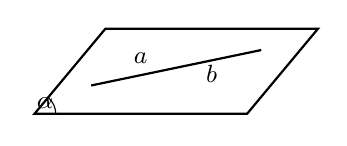
\begin{tikzpicture}[scale=0.9, >=stealth]
  \draw[thick] (0,0) -- (3,0) -- (4,1.2) -- (1,1.2) -- cycle;
  \draw (0.3,0) arc (0:50:0.3);
  \node at (0.15,0.15) {\small $\alpha$};
  \draw[thick] (0.8,0.4) -- (3.2,0.9);
  \node[above] at (1.5,0.57) {\small $a$};
  \node[below] at (2.5,0.82) {\small $b$};
\end{tikzpicture}
&
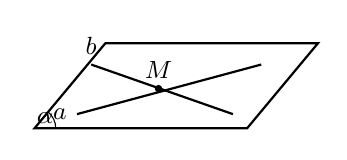
\begin{tikzpicture}[scale=0.9, >=stealth]
  \draw[thick] (0,0) -- (3,0) -- (4,1.2) -- (1,1.2) -- cycle;
  \draw (0.3,0) arc (0:50:0.3);
  \node at (0.15,0.15) {\small $\alpha$};
  \draw[thick] (0.6,0.2) node[left] {\small $a$} -- (3.2,0.9);
  \draw[thick] (0.8,0.9) node[above] {\small $b$} -- (2.8,0.2);
  \coordinate (M) at (1.75,0.56);
  \fill (M) circle (1.5pt);
  \node[above] at (1.75,0.56) {\small $M$};
\end{tikzpicture}
&
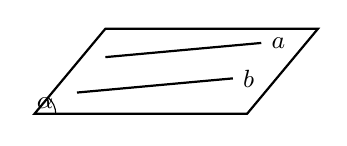
\begin{tikzpicture}[scale=0.9, >=stealth]
  \draw[thick] (0,0) -- (3,0) -- (4,1.2) -- (1,1.2) -- cycle;
  \draw (0.3,0) arc (0:50:0.3);
  \node at (0.15,0.15) {\small $\alpha$};
  \draw[thick] (1.0,0.8) -- (3.2,1.0) node[right] {\small $a$};
  \draw[thick] (0.6,0.3) -- (2.8,0.5) node[right] {\small $b$};
\end{tikzpicture}
&
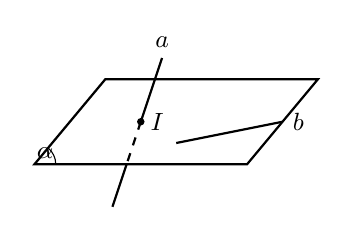
\begin{tikzpicture}[scale=0.9, >=stealth]
  \draw[thick] (0,0) -- (3,0) -- (4,1.2) -- (1,1.2) -- cycle;
  \draw (0.3,0) arc (0:50:0.3);
  \node at (0.15,0.15) {\small $\alpha$};
  \draw[thick] (2.0,0.3) -- (3.5,0.6) node[right] {\small $b$};
  \coordinate (I) at (1.5,0.6);
  \draw[thick] (1.8,1.5) node[above] {\small $a$} -- (I);
  \draw[dashed, thick] (I) -- (1.3,0);
  \draw[thick] (1.3,0) -- (1.1,-0.6);
  \fill (I) circle (1.5pt) node[right] {\small $I$};
\end{tikzpicture}
\\
$a \equiv b$ & $a \cap b = \{M\}$ & $a \parallel b$ & $a, b$ chéo nhau \\
a) & b) & c) & d)
\end{tabular}
\end{center}

\vspace{0.4cm}

\noindent\textbf{\color{myblue}{a/ Hai đường thẳng song song:}} nếu chúng cùng nằm trên một mặt phẳng và không có điểm chung.

\begin{notebox}
\noindent\textbf{\color{myred}{\textit{*Chú ý:}}}\\
\indent 1. Hai đường thẳng gọi là \textit{chéo nhau} nếu chúng không đồng phẳng.\\
\indent 2. Cho hai đường thẳng song song $a$ và $b$. Có duy nhất một mặt phẳng chứa hai đường thẳng đó, kí hiệu $\text{mp}(a, b)$.
\end{notebox}

\vspace{0.2cm}

\noindent\textbf{\color{myblue}{b/ Tính chất cơ bản về hai đường thẳng song song.}}\\
\textbf{+} Nếu ba mp phân biệt đôi một cắt nhau theo ba giao tuyến phân biệt thì ba giao tuyến ấy hoặc đồng quy hoặc đôi một song song với nhau.

\vspace{0.4cm}

% 2 Diagrams for 3 planes intersection
\begin{center}
\begin{tabular}{cc}
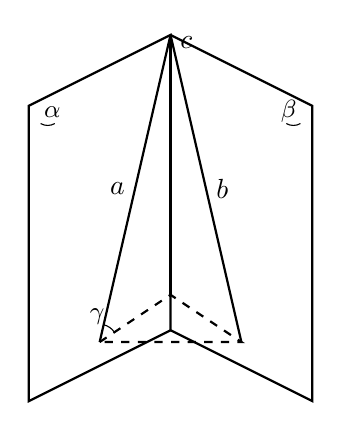
\begin{tikzpicture}[scale=1.5, >=stealth]
  % Coordinates of the book pages
  \coordinate (V) at (0,2);
  \coordinate (O) at (0,-0.5);
  \coordinate (TL) at (-1.2, 1.4);
  \coordinate (BL) at (-1.2, -1.1);
  \coordinate (TR) at (1.2, 1.4);
  \coordinate (BR) at (1.2, -1.1);

  % Draw left page (alpha)
  \draw[thick] (TL) -- (V) -- (O) -- (BL) -- cycle;
  % Draw right page (beta)
  \draw[thick] (V) -- (TR) -- (BR) -- (O);

  % Label alpha
  \draw (-1.1, 1.25) arc (240:300:0.12);
  \node at (-1.0, 1.35) {\small $\alpha$};
  
  % Label beta
  \draw (1.1, 1.25) arc (300:240:0.12);
  \node at (1.0, 1.35) {\small $\beta$};

  % Bottom points of the lines
  \coordinate (A0) at (-0.6, -0.6);
  \coordinate (B0) at (0.6, -0.6);
  \coordinate (C0) at (0, -0.2);

  % Dashed triangle (plane gamma)
  \draw[dashed, thick] (A0) -- (C0) -- (B0) -- cycle;

  % Draw the intersection lines a, b, c
  \draw[thick] (A0) -- (V) node[midway, left] {$a$};
  \draw[thick] (B0) -- (V) node[midway, right] {$b$};
  \draw[thick] (C0) -- (V);
  \node[above right] at (0, 1.8) {$c$};

  % Label gamma at A0
  \draw (-0.6, -0.6) + (34:0.15) arc (34:77:0.15);
  \node at (-0.62, -0.38) {\small $\gamma$};
\end{tikzpicture}
&
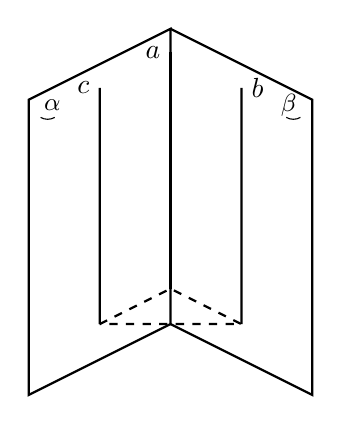
\begin{tikzpicture}[scale=1.5, >=stealth]
  % Coordinates of the book pages
  \coordinate (V) at (0,2);
  \coordinate (O) at (0,-0.5);
  \coordinate (TL) at (-1.2, 1.4);
  \coordinate (BL) at (-1.2, -1.1);
  \coordinate (TR) at (1.2, 1.4);
  \coordinate (BR) at (1.2, -1.1);

  % Draw left page (alpha)
  \draw[thick] (TL) -- (V) -- (O) -- (BL) -- cycle;
  % Draw right page (beta)
  \draw[thick] (V) -- (TR) -- (BR) -- (O);

  % Label alpha
  \draw (-1.1, 1.25) arc (240:300:0.12);
  \node at (-1.0, 1.35) {\small $\alpha$};
  
  % Label beta
  \draw (1.1, 1.25) arc (300:240:0.12);
  \node at (1.0, 1.35) {\small $\beta$};

  % Bottom points of the lines
  \coordinate (C0) at (-0.6, -0.5);
  \coordinate (B0) at (0.6, -0.5);
  \coordinate (A0) at (0, -0.2);

  % Dashed triangle (plane gamma)
  \draw[dashed, thick] (C0) -- (A0) -- (B0) -- cycle;

  % Vertical lines
  \draw[thick] (C0) -- (-0.6, 1.5) node[left] {$c$};
  \draw[thick] (B0) -- (0.6, 1.5) node[right] {$b$};
  \draw[thick] (A0) -- (0, 1.8) node[left] {$a$};
\end{tikzpicture}
\end{tabular}
\end{center}

\vspace{0.4cm}

\noindent\textbf{+} Nếu hai mp phân biệt lần lượt chứa hai đt song song thì giao tuyến của chúng (nếu có) cũng song song với hai đt đó hoặc trùng với một trong hai đt đó.

\vspace{0.4cm}

% 3 Diagrams for parallel lines in intersecting planes
\begin{center}
\begin{tabular}{ccc}
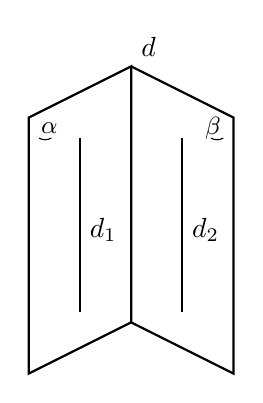
\begin{tikzpicture}[scale=1.3, >=stealth]
  \coordinate (V) at (0,2);
  \coordinate (O) at (0,-0.5);
  \coordinate (TL) at (-1.0, 1.5);
  \coordinate (BL) at (-1.0, -1.0);
  \coordinate (TR) at (1.0, 1.5);
  \coordinate (BR) at (1.0, -1.0);

  \draw[thick] (TL) -- (V) -- (O) -- (BL) -- cycle;
  \draw[thick] (V) -- (TR) -- (BR) -- (O);

  \draw (-0.9, 1.3) arc (240:300:0.12);
  \node at (-0.8, 1.4) {\small $\alpha$};
  \draw (0.9, 1.3) arc (300:240:0.12);
  \node at (0.8, 1.4) {\small $\beta$};

  \draw[thick] (0, -0.5) -- (0, 2) node[above right] {$d$};
  \draw[thick] (-0.5, -0.4) -- (-0.5, 1.3);
  \node[right] at (-0.5, 0.4) {$d_1$};
  \draw[thick] (0.5, -0.4) -- (0.5, 1.3);
  \node[right] at (0.5, 0.4) {$d_2$};
\end{tikzpicture}
&
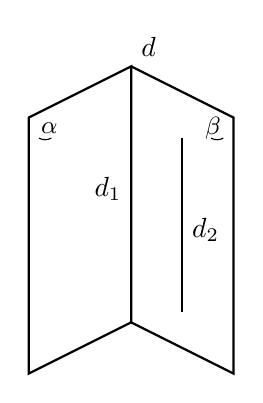
\begin{tikzpicture}[scale=1.3, >=stealth]
  \coordinate (V) at (0,2);
  \coordinate (O) at (0,-0.5);
  \coordinate (TL) at (-1.0, 1.5);
  \coordinate (BL) at (-1.0, -1.0);
  \coordinate (TR) at (1.0, 1.5);
  \coordinate (BR) at (1.0, -1.0);

  \draw[thick] (TL) -- (V) -- (O) -- (BL) -- cycle;
  \draw[thick] (V) -- (TR) -- (BR) -- (O);

  \draw (-0.9, 1.3) arc (240:300:0.12);
  \node at (-0.8, 1.4) {\small $\alpha$};
  \draw (0.9, 1.3) arc (300:240:0.12);
  \node at (0.8, 1.4) {\small $\beta$};

  \draw[thick] (0, -0.5) -- (0, 2) node[above right] {$d$};
  \node[left] at (0, 0.8) {$d_1$};
  \draw[thick] (0.5, -0.4) -- (0.5, 1.3);
  \node[right] at (0.5, 0.4) {$d_2$};
\end{tikzpicture}
&
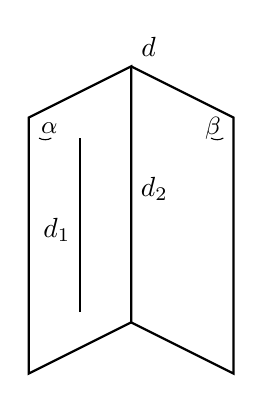
\begin{tikzpicture}[scale=1.3, >=stealth]
  \coordinate (V) at (0,2);
  \coordinate (O) at (0,-0.5);
  \coordinate (TL) at (-1.0, 1.5);
  \coordinate (BL) at (-1.0, -1.0);
  \coordinate (TR) at (1.0, 1.5);
  \coordinate (BR) at (1.0, -1.0);

  \draw[thick] (TL) -- (V) -- (O) -- (BL) -- cycle;
  \draw[thick] (V) -- (TR) -- (BR) -- (O);

  \draw (-0.9, 1.3) arc (240:300:0.12);
  \node at (-0.8, 1.4) {\small $\alpha$};
  \draw (0.9, 1.3) arc (300:240:0.12);
  \node at (0.8, 1.4) {\small $\beta$};

  \draw[thick] (0, -0.5) -- (0, 2) node[above right] {$d$};
  \node[right] at (0, 0.8) {$d_2$};
  \draw[thick] (-0.5, -0.4) -- (-0.5, 1.3);
  \node[left] at (-0.5, 0.4) {$d_1$};
\end{tikzpicture}
\\
a) & b) & c)
\end{tabular}
\end{center}

\vspace{0.4cm}

\noindent\handwrite\ \textbf{\color{myblue}{+ Hai đường thẳng phân biệt cùng song song với đường thẳng thứ ba thì song song với nhau.}}
\[
\begin{cases}
a \neq b \\
a \parallel c \\
b \parallel c
\end{cases}
\Rightarrow a \parallel b
\]

\end{document}
